\documentclass{article}
\usepackage[utf8]{inputenc}
\usepackage{changepage}% http://ctan.org/pkg/changepage for adjustwidth
\usepackage{amsmath}
\usepackage{amsfonts} 
\usepackage{amssymb}
\usepackage{hyperref}
\usepackage{graphicx}
\usepackage{minted}
\usepackage[T1]{fontenc}
\usepackage[margin=0.9in]{geometry}
\renewcommand*\familydefault{\sfdefault} %% sans serif
\setlength{\parindent}{0pt}
\def\code#1{\texttt{#1}}
\def\member{$\in$ }
\def\wholeNumbers{\mathbb{W}}
\def\expected{\mathbb{E}}
\def\suchThat{\hspace{0.5em} s.t. \hspace{0.5em}}
\def\s{\hspace{0.3em}}


%
% Commands
%

\newcommand{\br}{ \hfill \break}

% setup for blocks of code (use \begin{lstlisting})
\usepackage{listings}
\usepackage{color}
\definecolor{dkgreen}{rgb}{0,0.6,0}
\definecolor{gray}{rgb}{0.5,0.5,0.5}
\definecolor{mauve}{rgb}{0.58,0,0.82}
\lstset{
  frame=tb,
  language=Json,
  aboveskip=3mm,
  belowskip=3mm,
  showstringspaces=true,
  columns=fixed,
  basicstyle={\small\ttfamily},
  numbers=none,
  numberstyle=\tiny\color{gray},
  keywordstyle=\color{blue},
  commentstyle=\color{dkgreen},
  stringstyle=\color{mauve},
  breaklines=false,
  breakatwhitespace=false,
  tabsize=3
}


% Head

\title{Progress Log}
\author{Jeff Hykin}
\begin{document}
\maketitle
% 
% Body
% 


% 
% Finding Happiness Draft 1
% 
\date{July 20,21,22 2020} \br \begin{adjustwidth}{2.5em}{0pt}
\section{Finding Happiness}

    \subsection{Problem Definition}
        Consider a video with an infinte sequence of frames, where $i$ represents the index of the frame.
        \begin{align*}
            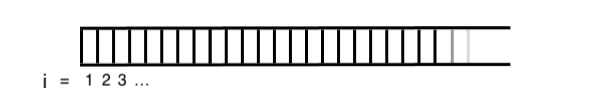
\includegraphics{infinite_frames.png}
        \end{align*}
        
        Suppose there is a high-cost algorithm $H(i)$ that is equal to 1 if the frame at index $i$ is a "hit" and is otherwise equal to 0.
        For our particular case, a hit means a face with a happy expression was found in the frame corrispoding to index $i$,
        however a hit need not mean something so specific.\br 
        \br 
        The general problem we hope to solve here is finding an algorithm $A(n)$ that maximizes the number of hits while minimizing the number of calls to $H(i)$.
        This is represented formally as:
        $$n: the\ number\ of\ calls\ to\ H(i)$$
        $$A(n): \wholeNumbers \mapsto \{\s   i   \s|\s   H(i) = 1 \s\} $$
        $$S(n): max( \displaystyle\frac{|\s A(n) \s|}{n} )$$
        
        Additionally, suppose that $H(i)$ caches all values, such that, for a particular $i$, subsequent calls to $H(i)$ are considered to have a $O(1)$ runtime.
        Let $C(j)$ be the set of indicies that have been cached at a particular iteration $j$. Finally, we approach this problem as the challege of selecting the
        index $i$ that has the highest probability of being a hit, given the cache $C(j)$.
    
    \subsection{Random Sampling}
        
        Seeing as probabilies cannot be be infered without some form of prior knowledge, here we define a sampling method $R(q,w)$ to be used in following sections.\br
        \br
        Given the infinite sequence of frames 
        \begin{align*}
            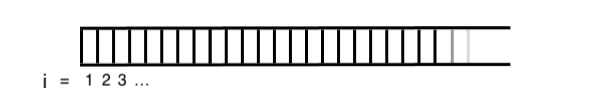
\includegraphics{infinite_frames.png}
        \end{align*}
        Let there be a sampling method $R(q,w)$, where $q$ is the quantity of samples, and $w$ is the cardinality (or "width") of each sample.\br
        For example: (note: graphics are a draft)
        \begin{align*}
            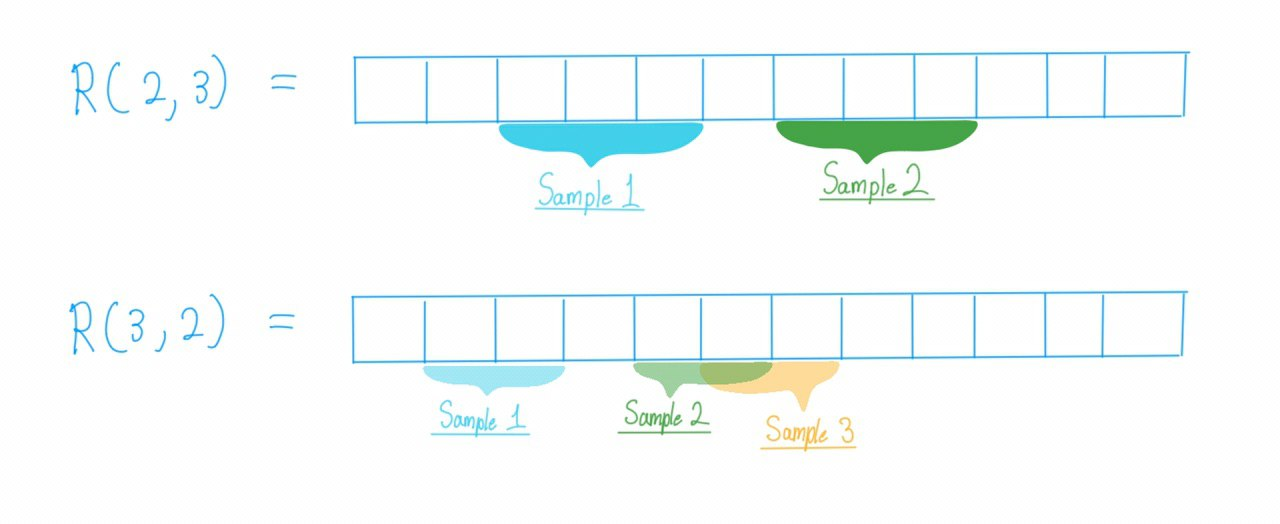
\includegraphics[width=\textwidth,height=\textheight,keepaspectratio]{random_sample_examples.jpeg}
        \end{align*}
        The method $R(q,w)$ returns a set of sub-sequeces which we can consider as samples from the population $\phi(w)$ which represents all sub-sequeces of length $w$.
        Additionally let all indicies in all sequences of R(q,w) be presumed to have been cached, either before or durning the runtime of $A(n)$.
    
    \subsection{Core Probability Estimation}
        The goal is to efficiently find the index with the highest probability of a hit.
        Here we address the core use of binomial statistics to estimate the probablilty that a single index $i_\alpha$ is a hit.\br
        \br
        To accomplish this, several values are temporarily assumed to be convenient givens.
        Note that the calculation of each of these are the respective topics of following sections.
        These temporary givens are:
        \begin{itemize}
            \item an iteration $j_\alpha$
            \item a non-cached index $i_\alpha$, $i_\alpha \notin C(j_\alpha)$
            \item a fixed sample quantity $q_\alpha$
            \item a fixed sample width $w_\alpha$
            \item a given sub-sequence $M_\alpha$, $i_\alpha \in M_\alpha$, $|M_\alpha| = w_\alpha$
        \end{itemize}
        These will be eventually be replaced by their respective variable counterparts
        \begin{itemize}
            \item $j_\Omega$
            \item $i_\Omega$
            \item $q_\Omega$
            \item $w_\Omega$
            \item $M_\Omega$
        \end{itemize}
        
        \br
        The calculation of $P( H(i_\alpha) = 1 )$ can be taken from the expected probablilty that any randomly selected index from $M_\alpha$ is a hit.
        This probability will be defined as teh expected hit rate of $M_\alpha$. The true hit rate of $M_\alpha$ is defined as
        $$ \mathit{HR}(M_\alpha) = \displaystyle\frac{\displaystyle\sum_{i \in M_\alpha}^{} H(i) }{|M_\alpha|} $$
        The issue here is that not all the hit values of $M_\alpha$ are known. To estimate this hit rate, we use random sampling.
        Since $q_\alpha$ is conveniently defined as a given, we use all of the $q_\alpha$ samples from $R(q_\alpha, w_\alpha)$ to form a distribution of hit rates $D(q_\alpha, w_\alpha)$ as follows:
        $$ D(q_\alpha, w_\alpha) = [ \mathit{HR}(x) | x \in R(q_\alpha, w_\alpha) ] $$
        By treating the cached indices of $M_\alpha$, formally $M_\alpha \cap C(j_\alpha)$, as a Bernoulli process,
        and by treating $d \in D(q_\alpha, w_\alpha)$ as a Bernoulli distribution, we can calculate the probablilty of $M_\alpha$ being a sample taken from $d$, $P(M_\alpha | d)$, as follows.
        $$ P_D = \displaystyle\sum_{d \in D(q_\alpha, w_\alpha)}^{} P(M_\alpha | d) $$
        $$ \expected(\s    \mathit{HR}(M_\alpha)    \s|\s     D(q_\alpha, w_\alpha)    \s) =  \displaystyle\sum_{d \in D(q_\alpha, w_\alpha)}^{} d * \displaystyle\frac{P(M_\alpha | d)}{P_D}  $$
        
        With this in hand, the initial interest of this section can be written as:
        $$ P( \s H(i_\alpha) = 1 \s|\s M_\alpha, q_\alpha, w_\alpha, C(j_\alpha) \s) = \expected(\s    \mathit{HR}(M_\alpha)    \s|\s    D(q_\alpha, w_\alpha)    \s) $$
    \section{Selection of $M_\Omega$}
        Here we address the optimal selection of a sequence $M$ that maximizes the statistical accuracy of $P(\s H(i_\alpha) = 1 \s|\s M, q_\alpha, w_\alpha, C(j_\alpha) \s)$
        \br\br
        Similar to the last section, we temporarily assume the follow as givens
        \begin{itemize}
            \item an iteration $j_\alpha$
            \item a non-cached index $i_\alpha$, $i_\alpha \notin C(j_\alpha)$
            \item a fixed sample quantity $q_\alpha$
            \item a fixed sample width $w_\alpha$, s.t. $|M| = w_\alpha$
        \end{itemize}
        
        For the sake of illustration, consider the following where:
        \begin{itemize}
            \item The blue arrow indicates $i_\alpha$
            \item The green dots indicate indicies where $H(i) = 1$
            \item The red dots indicate indicies where $H(i) = 0$
            \item The gray dots indicate indicies that are not yet cached
        \end{itemize}
        (note illustration is a draft/stand-in)
        \begin{align*}
            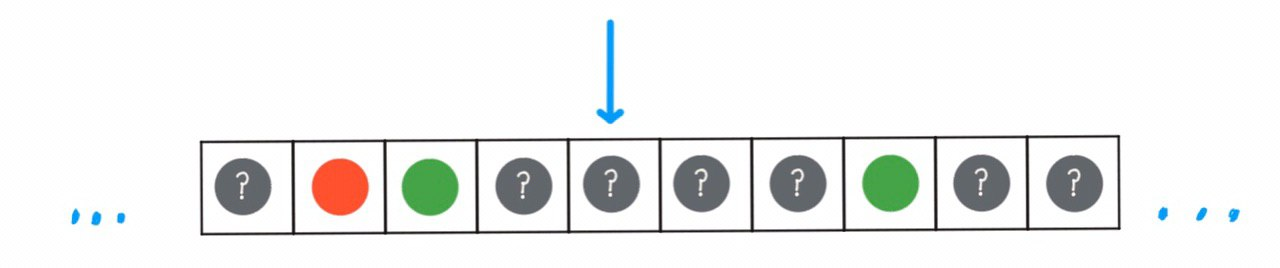
\includegraphics[width=\textwidth,height=\textheight,keepaspectratio]{sequence_sample.jpg}
        \end{align*}
        
        Given that $i_\alpha \in M$, and supposing that $w_\alpha = 4$ the possible sequences of M can be represented visually as:\br
        (note illustration is a draft/stand-in)
        \begin{align*}
            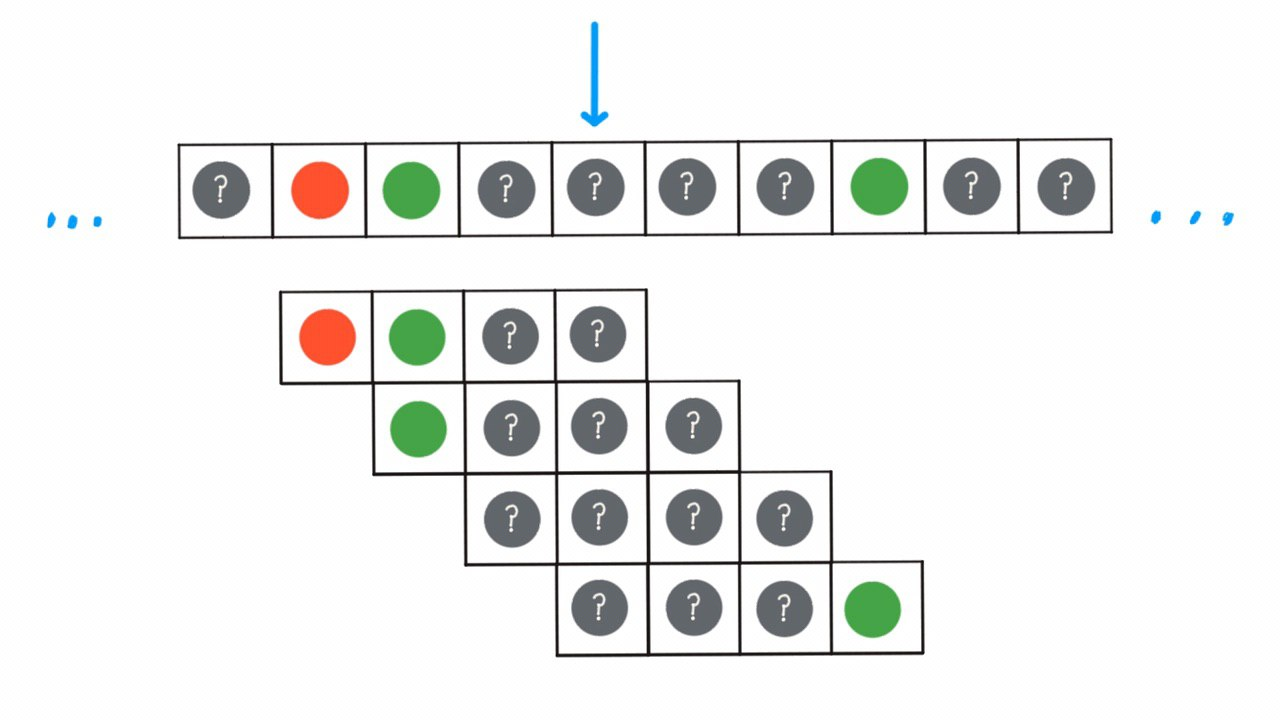
\includegraphics[width=\textwidth,height=\textheight,keepaspectratio]{sequence_sample_slices.jpg}
        \end{align*}
        
        Here we define a measure of statistical relevancy refered to as strength.
        Not to be confused with any pre-existing statistical use of the term.
        Strength is defined as $\delta(x)$ where $x$ can be any sequence of indicies
        $$\delta(x) = \displaystyle\frac{|C(j_\alpha)|}{|x|}$$
        Applying this to the above illustration would result in:\br
        (note illustration is a draft/stand-in)
        \begin{align*}
            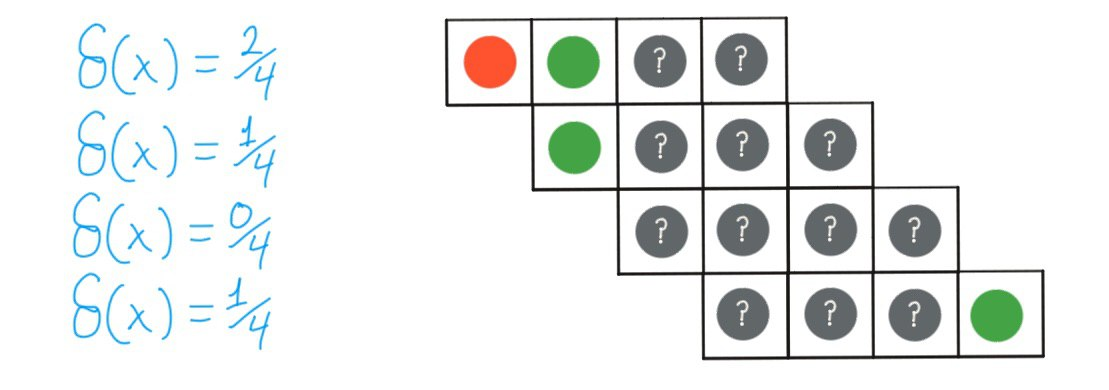
\includegraphics[width=\textwidth,height=\textheight,keepaspectratio]{samples_with_strength_label.jpg}
        \end{align*}
        The simple description is to select the sequence with the highest strength as the ideal $M$.
        However, in the case of a tie all of the sequences with the highest power should be selected and their probabilities averaged.
        This means $M_\Omega$ is not a sequence but a set of sequences, often containing only one element.\br\br 
        
        The calculation of $M_\Omega$ can be written formally as:
        $$M_\Omega = \{\s   x   \s|\s   i_\alpha \in x, x \in \phi(w_\alpha)   \s\}$$
        $$\bar{\delta} = \mathit{max}(\{\s   \delta(M)   \s|\s   M \in M_{i_\alpha}   \s\})$$
        $$M_\Omega = \{\s  M  \s|\s  \delta(M) = \bar{\delta}, M \in M_{i_\alpha} \s\}$$
        The probability $P(\s H(i_\alpha) = 1 \s)$ can be improved from
        $$ P(\s   H(i_\alpha) = 1   \s|\s   M_\alpha, q_\alpha, w_\alpha, C(j_\alpha)   \s) = \expected(\s    \mathit{HR}(M_\alpha)    \s|\s    D(q_\alpha, w_\alpha)    \s) $$
        To 
        $$ P(\s   H(i_\alpha) = 1   \s|\s   q_\alpha, w_\alpha, C(j_\alpha)   \s) = \mathit{mean}([ \expected(\s    \mathit{HR}(M)    \s|\s    D(q_\alpha, w_\alpha)    \s) | M \in M_\Omega ])$$
        
        \br\br
        Note, with concern to the time complexity of $M \in M_\Omega$, a cache can be formed.
        Rather than each $M$ having a cached value, $M$ can be converted into an unordered list.
        This reduces the size of teh cache from having a space complexity of all binary permutations
        of size $w_\alpha$ to the smaller space of all binary combinations of size $w_\alpha$. Which
        will effectively reduce the runtime of $|M_\Omega|$ to a size dramatically smaller. See the 
        following sections as to how caches with such large space complexity are pratical by side
        effects of choosing an optimal $w_\alpha$.
        
\end{adjustwidth} \br

\date{July 9th 2020} \br \begin{adjustwidth}{2.5em}{0pt} 
\section{Finding Happiness}

    \subsection{Problem Definition}
        Consider a video with infinite sequence of frames, where each frame is enumerated with an index $i \hspace{0.3em}s.t.\hspace{0.3em} i \in I,\hspace{0.3em} I \subseteq \wholeNumbers $. Suppose, in addition to being infinite, that any frame can be accessed in a constant amount of time.
        \begin{align*}
            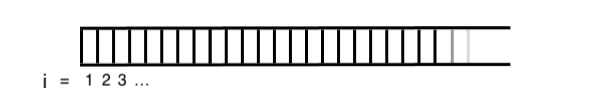
\includegraphics{infinite_frames.png}
        \end{align*}
        In this scenario $H(i)$ is a function $ H: \wholeNumbers \mapsto \{0,1\} $ where
        \begin{adjustwidth}{2.2em}{0pt}
            $H(x) = 1$ indicates a frame is a "hit" \\ 
            $H(x) = 0$ indicates a frame is a "miss" \\
        \end{adjustwidth}
        In our particular application we define a "hit" as a frame containing a face with a happy expression.\br
        Ideally an algorithm $A(n)$ would iteratively select the index with the highest likelihood of being a hit, with $n$ being the number of iterations. This algorithm would return a set of indices $i_a \in A(n)$, where each index was a hit $\forall i_a, H(i_a) = 1$. The problem is framed as maximizing the score of an algorithm $S(A, n)$, which is defined as the proportion of hits per iteration\br

            $$ S(A, n) = \frac{ \displaystyle\sum^{i \in A(n)} H(i) }{ n }$$ \\

        In addition to this, it is also desirable to minimize the size of the largest index $k$ that is accessed, as a measurement of "wasted" frames defined as $W(n)$.

            $$ k \in A(n) \suchThat k \leq a, \forall a \in A(n) $$
            $$ W(n) = \displaystyle\sum_{j=1}^{k} H(j) - S(A, n) $$ \\
        
    
    \subsection{Building Probability Distributions}
        To generate the probability of a hit $P_H(i)$ for an index $i$, we must work to answer a few questions.
        \begin{itemize}
            \item What is $P_H(i)$, given no other information?
            \item What is $P_H(i)$, given a nearby frame is a hit?
            \item What is $P_H(i)$, given a nearby frame is a miss?
            \item What is $P_H(i)$, given $c_h$ adjacent hits?
            \item What is $P_H(i)$, given $c_m$ adjacent misses?
        \end{itemize}
        Before making any statistical inferences, at least some prior data will be needed. Suppose sub-sequences of various lengths are taken from the video and put into a set $R$. (Suppose also that these sequences are a representative random sample, and that the hit/miss value has been pre-found for every frame in every sub-sequence.)
        \br
        \br
        To answer the first question, each sequence in $R$ must be broken down into a set of 1-frame sequences, represented as $F_1$. The probability is then found as the hit ratio $\mathit{HR}$ of the set of frames $HR(F_1)$
            $$ \mathit{HR}(X) =  \frac{ \displaystyle\sum^{i \in X} H(i) }{ |X| }  $$
        
        As for the subsequent questions, lets consider an example of these sequence sets $F_1, F_2, F_4$.
        \begin{lstlisting}
F_1 = {  [ 12233 ],                   [ 1 ],       [ 9 ],           }
F_2 = {  [ 12233,12234 ],             [ 1,2 ],     [ 9,10 ],        }
F_4 = {  [ 12233,12234,12235,12236 ], [ 1,2,3,4 ], [ 9,10,11,12 ],  }
        \end{lstlisting}
        (Note, sets with sequences with a count larger than 1 need a method of selection, but we will not address that here.)\br
        For each of these sets $F_j \in F$, lets build a corresponding distribution $D_j \in D$. This can be done by replacing each sequence with the hit-ratio of all indices in that sequence.
        \begin{lstlisting}
D_1 = [  0,       1,    1,  ] # assuming H(12233)=0, H(1)=1, H(9)=1
D_2 = [  0.5,     0.5,  1,  ] # assuming H(12234)=1, etc
D_4 = [  0.75,    0.25, 1,  ] # etc
        \end{lstlisting}
        Mathematically represented as
        $$ D_j = [ x | x = \mathit{HR}(s), \forall s \in F_i  ]  $$
        Given these distributions corresponding to sequences of length $i$, we can now move on.
        
    \subsection{Calculating Probabilities}
        Given that we have a $c_h$ close-by hits, and $c_m$ close-by misses, we can determine a distribution $D_k$ that would be most suited for prediction. Before this is done however, consider the following analogy.\br\br
        
        Instead of merely a ratio, imagine each elment of $D_k$ to be a bag containing $k$ marbles. Given that the bag has a ratio, imagine that ratio $b_r$ as indicating the bag's ratio of green and red marbles, green representing a hit and a red representing a miss. Similarly consider $c_h$ as a quantity of green marbles, and $c_m$ a quantity of red marbles.\br\br
        
        By treating each bag as a binomial distribution, we can compute $P_d(b)$ as the likelihood that $c_h$ and $c_m$ were drawn from each bag $b \in D_k$.
                    $$ P_d(b) =  b_r^{(c_h)} * (1-b_r)^{(c_m)} $$
        
        These binomial probabilities can then be normalized and used as weights for each ratio. 
                    $$ P_\mathit{total} = \displaystyle\sum^{\forall b \in D_k} P_d(b) $$
                    $$ P_H(i | D_k, c_h, c_m) = \displaystyle\sum^{\forall b \in D_k} b_r * ( P_d(b) / P_\mathit{total} )  $$
        
        In light of the analogy, the task of selecting a $D_k$ is simplified to selecting the ideal bag-size $k$. Given that we are asking for the probability that $c_h$ green, $c_m$ red, and one unknown $i$ are being drawn from a bag, $k$ should at least be $k \geq c_h + c_m + 1$. To gain the highest accuracy possible, it would also be ideal to minimze the number of unknown marbles, meaning $k = c_h + c_m + 1$. If such a $D_k$ is not avaible, then the next closest ideal is $min(|k - (c_h + c_m + 1)|)$.
    
    \subsection{Infinte Comparison}
        Finding the frame with the highest likelihood $i_m$ by comparing against all frames in an infinitely long video might be considered computationially expesive. Thankfully, convergence and the Law of Large Numbers, allows us to sidestep this problem entirely. As the sequence size $k$ increases, the ratios in $D_k$ are guarenteed to converge on the population ratio of the entire video. Since the frame with the highest probability is the only one of interest, the confidence needed for convergence towards the average probablilty can be relatively low. This provides both a theoretical and pratcial bound $w$ for creating $|D| = w \suchThat D_j \in D$.
        
    \subsection{Time Complexity and Optimization}
        The time complexity of $A(n)$ is then $O(n * (O(H) + m))$ where $n$ is the number of iterations, $m$ is the size of the largest $D_j$, and $O(H)$ is the time complexity of the hit detection function. A tradeoff can be made to reduce $m$ to nearly $1$ at cost of space complexity. This is done by caching the results of $P_H(i | D_k, c_h, c_m)$, until all common combinations needed for convergence have been cached.
    
    \subsection{Python Implmentation}
        \begin{minted}[]{python}
def probability_of_belonging(good_frame_count, bad_frame_count, ratio):
    return (ratio ** good_frame_count) * ((1-ratio) ** bad_frame_count)

def weighted_probability(good_frame_count, bad_frame_count, distribution):
    likelihoods = [ probability_of_belonging(number_of_hits, number_of_misses, each) for each in distribution ]
    total = sum(likelihoods)
    # normalize likelihoods to use them as weights
    likelihoods = [ each / total for each in likelihoods]
    weighted_amounts = [ each_ratio * each_likelihood for each_ratio, each_likelihood in zip(distribution, likelihoods) ]
    return sum(weighted_amounts)

def get_distribution(bucket_size, video_frame_labels):
    distribution = []
    start = 0
    end = bucket_size
    while end < video_frame_labels:
        start += bucket_size / 2
        end += bucket_size / 2
        segment = video_frame_labels[start:end]
        distribution.append((sum(segment)+0.0)/len(segment))
    
    return distribution


def get_distribution(videos):
    buckets = []
    distribution = []
    for index in range(2,100):
        bucket_size = index
        distribution = []
        distribution.append(distribution)
        for each in videos:
            distribution += get_distribution(bucket_size, videos.frame_labels)
    
# 
# example
# 
number_of_misses = 2
number_of_hits = 2
distribution_5 = [
    0.93,
    0.92,
    0.91,
    0.90,
    0.50,
    0.10,
    0.09,
    0.08,
]
print('sum(weighted_amounts) = ', weighted_probability(2, 2, distribution_5))
        \end{minted}
    
    \subsection{Conclusion}
        ((TODO))
        ((future idea: localized, or "forgetful" statistics))
        

%
%
\end{adjustwidth} \br
%
\date{June 21 2020} \br \begin{adjustwidth}{2.5em}{0pt}
\#\br
\#\br
\# Finding Faces and the Game of Battleship \br
\#\br
\#\br
\br
Optimally finding frames containing faces may seem unrelated to the board game of Battleship. The key hides in the pedestrian observation that frames with faces most often occur in sequences. For empirical validity, this was confirmed based on a data set of 360 randomly selected videos. The mapping between these two problems is quite useful since the game of Battleship is known to have a mathematically optimal strategy for winning, as shown in the article "Battleship and the Negative Hypergeometric Distribution" by Melanie A. Autin and Natasha E. Gerstenschlager. In the game of Battleship, each player has a 10x10 grid of cells along with ships of various lengths that can be placed on the grid. The players take turns guessing the locations of the opponent's ships, one cell at a time. A sequence of frames containing faces can be thought of as a ship, and the video itself can be thought of as a one dimensional grid. The downside is that, with videos, the ships are of an unknown length, and unknown quantity. On the upside however, the videos don't shoot back. Having a minimum ship length of one, combined with an unknown number of ships, requires a player to guess every possible cell before declaring absolute victory. Thankfully enough however, the case of video processing does not need to find every last rowboat and buoy. If we increase the minimum ship length to merely two units, the absolute victory condition goes from needing every cell, to only needing every-other cell. A minimum duration of 1 second (approximately 32 frames) would likely be useful for training machine learning models. And, with that minimum ship size of 32, along with a single-dimension grid, the game becomes orders-of-magnitude easier to win. Not only in terms of never missing any major ships, but also in terms of having the highest possible ratio of hits per guess.\br
\br
Optimizing the game of Battleship requires applying a probability density function to every cell in the grid. This involves simulating every possible permutation of all ships in order to find the cells with the highest probability of containing a ship. The end result is that center of the grid (e.g. video) will always be selected as the most likely spot. This is because ships have fewer possible configurations involving only edge-cells, with many more possible ways of being placed in cells closer to the center. After choosing the middle frame, a miss would cause a cascading reduction in the probability of all nearby cells. Furthermore, the sum total of probabilities from all cells would also drop because it is certain that a ship spanning the whole grid (or even just half of the grid) cannot be not present. Supposing that the initial guess is a hit however, would cause the exact inverse reaction. Nearby cells would cascadingly increase in probability, and the sum total of probabilities for the video as a whole will rise significantly. This process can then be repeated continually by always selecting the cell with the highest probability.\br
\br
\# Higher Order Battleship\br
\br
The macro process of finding faces is not a single game of Battleship but instead one game of Battleship per video, all of which are (theoretically) being played simultaneously. If the outcome of a particular game is looking grim, simply start (or resume) a different game. More specifically, if the highest probability of a hit in a particular video is lower than the probability of a hit on a new video, then a new video should be evaluated instead. Beyond this improvement, the average sizes and frequencies of ships can also be empirically estimated as more data is gathered, allowing for an increasingly accurate probability density function. A second-order game of Battleship can also be played by evaluating the probability of ships being near other ships. Most notably, this method can provide an empirical estimation of its own efficiency without needing to be trained on a large data set.\br
\br
\# Implementation\br
\br
A practical implementation of these strategies however, will be much more difficult than it may first appear. Some videos are actually the same image on every frame, or the same image but merely translated or rotated. This will cause face detections on every frame even when the video is undesirable. The probability of inaccurate reporting, such as reporting a miss when it was in fact a hit, will also need to be taken into account. There are likely many other practical barriers yet to be discovered.

\end{adjustwidth} \br


%
%
%
\date{June 18 2020} \br \begin{adjustwidth}{2.5em}{0pt}

Through the code in this repository we provide access to a undirected graph \code{G = (V, E) }  of YouTube links. Each node \code{v \member V} is a YouTube video, and each edge \code{e \member  E} is a relationship to a related video. For every video \code{v}, in addition to edges, we also provide access to the duration, frame-rate, and frame-data. The graph is stored using a hash map where each key is a unique video ID provided by YouTube. The number of nodes \code{|V|} in this graph is growing, but can be expected to be in the thousands. The average number of edges per node \code{|e|} is approximately 22. The details of how to explore the graph are explained in the following source: \br
https://github.com/jeff-hykin/iilvd\_interface/blob/master/README.md

\end{adjustwidth} \br

%
%
%
\date{June 16 2020} \br \begin{adjustwidth}{2.5em}{0pt}
A 3 page installation/setup/usage guide was created for A\&M students to be able to be able to use the video database. The guide is here: \br
https://github.com/jeff-hykin/iilvd\_interface/blob/master/README.md
\end{adjustwidth} \br

%
%
%
\date{June 15 2020} \br \begin{adjustwidth}{2.5em}{0pt}
The database has now been running on the GPU server with GPU optimizations, which is approximately x8 faster than before. Statistical logging was added to monitor the process as it unfolded.

Download Time: 1\% of duration
Download Size: ~7.2 Mb per minute of duration

Time spent finding faces:		(46\%) 138 sec per 5 min of video
Time spent finding emotion: 	(22\%) 66 sec per 5 min of video
Time spend saving to DB:		(19\%) 57 sec per 5 min of video
Other code (13\%)
\end{adjustwidth} \br




%
%
%
\date{June 13th 2020} \br \begin{adjustwidth}{2.5em}{0pt}
The collection system has now been fully running for 48 hours on my local machine. At the current average rates, it will be 17 days before 1000 videos has been collected. The code is running without GPU optimizations, and there are several opportunities for major improvements.
\end{adjustwidth} \br


%
%
%
\date{June 9 2020} \br \begin{adjustwidth}{2.5em}{0pt}
The system for continually labeling videos is now put in place. The process is as follows:\br 
- A priority system for collecting videos is established\br
- Videos are served in a stream-like fashion via python generators\br
- Videos are downloaded as .mp4 files as needed\br
- Each frame of the video is analyzed individually\br
- Using dlib detectMultiScale, all faces in a frame are discovered\br
- Light preprocessing is performed on the cropped face images\br
- The processed images are then run through 9-scale emotion detection model\br
- The predicted probabilities for all 9 emotions are recorded\br
- That data is then saved, over the network, to the database\br
\br
The system has been tested on various individual data, but requires a day or more of testing before being given the chance to run continually and possibly corrupt the entire database. There is a current format for saving data, however will be updated to better fit with additional data. Also note the emotion detection model used was obtained from a fellow researcher in the Information Innovation Lab.
\end{adjustwidth} \br

%
%
%
\date{June 7\&8 2020} \br \begin{adjustwidth}{2.5em}{0pt}
Work was completed on a dynamic video caching and selection system for getting videos into the emotion detection model. The selection system works as a class `VideoSelector` that can be given priorities of which videos to retrieve first. For example, `VideoSelector().is\_downloaded.has\_related\_videos.retrieve()` will return a generator that only outputs videos matching that criteria. That example only has a single priority. This example: \br `VideoSelector().is\_downloaded.then.has\_related\_videos.retrieve()` has two priorities, the first one is downloaded videos. Once the list of downloaded videos is exhausted it falls back on its second priority, which is videos that are related to some other videos. Every video that is not already downloaded is automatically downloaded before being returned. This system should be flexible enough to allow for dynamic queues in the future, where videos are ordered based on the evolving likelihood of each video's usefulness. 
\end{adjustwidth} \br

%
%
%
\date{June 4\&5 2020} \br \begin{adjustwidth}{2.5em}{0pt}
Updated the database to both be crash-tolerant and reactively update to changes in the code. The query code was improved and now all of the \href{https://docs.mongodb.com/manual/reference/operator/query/#query-selectors}{\underline{MongoDB query selectors}} are supported directly in both Ruby (data scraping) and Python (machine learning). This will allow for the next step of quantifying statistics about the data, and validation of data.
\end{adjustwidth} \br


%
%
%
\date{June 2 2020} \br \begin{adjustwidth}{2.5em}{0pt}
The related video collection script ran successfully for over 24 hours. In that time it exhausted the videos that were in the database and provided relations for 66,074 videos. Code for querying the database was added, and work was done towards data-validation.
\end{adjustwidth} \br

%
%
%
\date{June 1 2020} \br \begin{adjustwidth}{2.5em}{0pt}
Code was created and tested for recording related\_videos. Collected 21218 samples that contain related video data. Validation of data still needed. There are approximately 20 related videos (edges) per video. Current video data format is as follows, loosely following the YAML format.

\begin{lstlisting}
# null means not-yet-checked or unknown
# false means known-to-be-false: aka unavailable
(youtube_video_id): !map_or_null_or_false
    basic_info: !map_or_null
        duration: !seconds (duration)
        fps: !integer (fps)
        height: !pixels (height)
        width: !pixels (width)
        download_error: !true_or_null (download_error)
        
    related_videos: !map_or_null
        !string (related_video_id): {}  # this is a key-value pair
                                        # because there are different 
                                        # kinds of relationships
    
    facedata_1.2: !map_or_null
        good_faces: !bool_or_null (significant_number_of_big_faces)
        is_picture: !bool_or_null (all_checked_frames_equal)
        max_repeated_face: !integer (lots_of_same_person_or_no)
    
    frames: !map_or_null # this is a map instead of an array because 
                         # not all frames (indices) are checked
        !integer (frame_index):
            facedata_1.2: 
                big_faces_>=1: !true_or_false (frame_contained_good_face)
                faces: !list
                    - "is_big?": !true_or_false
                        "x": !integer (x_position_pixels)
                        "y": !integer (y_position_pixels)
                        "width": !integer (width_pixels)
                        "height": !integer (height_pixels)
\end{lstlisting}
\end{adjustwidth} \br


%
%
%
\# \br
\# \br 
\# Database Design and Implementation \br
\# \br 
\# \br
\date{May 25 2020} \br
\begin{adjustwidth}{2.5em}{0pt}

\begin{Overview}
    This entry covers the mathematical structure, the computer science data structure, time complexities, the API implementation, and finally the software implementation of the database of videos being used. 
\end{Overview}

\section{Theoretical Structure}

The data can be thought of as an undirected graph, where each video is a node and the edges are relationships to other videos. To implement this structure, a hash map is used. Each key in the mapping is a video id, the one provided by YouTube, and the value is a nested hash map and array structure. Here is the structure represented in a JSON-like format:

\begin{lstlisting}
{
    video_1_unique_key: {
        "related_videos": {
            video_2_unique_key: null
        }
    },
    video_2_unique_key: {
        "related_videos": {
            video_1_unique_key: null
        }
    }
}
\end{lstlisting}

This structure allows for O(1) retrieval times for any node or immediate neighbor, at the cost of having the memory overhead of edges * 2. Which is justifiable since storage is cheap and time is not nearly as cheap. Note that the edges themselves are key-value pairs. This allows for adding future properties such as relationship distance/strength or adding relationship qualities, such as being related in color scheme or being related in transcription/audio content.

\section{Software Implementation}

This information is for those interested in reading, reproducing, or otherwise using the code. The hash map structures were additionally chosen in order to house additional (unknown) information about the video. Because of this unknown structure, the noSQL database MongoDB was chosen.

GLFS (git large file storage) is used to handle the database files, which are currently stored within the git repo itself. This will likely change if there is any collaboration on the database, but it is ideal to store it locally for a single user. Docker is used to ensure compatibility with all OS's. Within docker containers a MongoDB service is created locally, and a Node.js server is run locally to create easy API for the MongoDB service. By using the API created by Node.js, videos can be added, retrived by id, edited, or deleted by anyone on the local network.

Videos that are are on que, but do not have details are stored as a null value (instead of a hash map). Videos that have been attempted, but are unavalible (such as being deleted) are stored as a false value instead of a null value or hash map. All successful videos with downloaded details will be a hash map.


\end{adjustwidth} \br 



%
%
%
\# \br
\# \br 
\# PowerPoint Script/Draft \br
\# (the concept machine) \br 
\# \br
\date{April 20 2020} \br
\begin{adjustwidth}{2.5em}{0pt}



\section{Overview}

- \textbf{Need:} Recognition without examples is hard and common\br
- \textbf{First Obstacle:} Adversarial attacks and systematic weaknesses\br
- \textbf{Second Obstacle:} Meta learning and plasticity\br
- \textbf{Solution:} A recursive network of concepts\br

\section{The Situation: The Tragedy of Alex}

Dr. Bach Prahp is a biomedical researcher and his assistant, Alex Nat, joined his lab a few months ago. \br

Dr. Bach needs Alex to identify WhatchaMaCallIt. This shouldn't be challenging as Dr. Bach can recognize WhatchaMaCallIt without fail. It just so happens that Dr. Bach doesn't have any examples with WhatchaMaCallIt on hand. However, after 1,000,000 attempts, Alex has failed to show Dr. Bach any data related to WhatchaMaCallIt. If only there were some way Dr. Bach could explain to Alex what WhatchaMaCallIt was. \br

Alas, no such way existed. So Dr. Bach told Mr. WhatchaMaCallIt that the assistant was unable to find any of his records. \br
 
\section{Obstacle 1: Backpropagation Didn't Slay the Hydra}

Explaining to Alex that WhatchaMaCallIt was a person seems to be obvious step, but on the contrary, Alex is a machine. Teaching the Alex-machine what a person is likely means teaching it about faces, limbs, clothing, and each of those concepts would need their own recursive explanations. While it may seem that backpropagation has solved this recursive problem, the work done with adversarial attacks shows that the recursive Hydra was partially side stepped.

*turtle vs shotgun*

*human definition of a gun*
*human definition of a turtle*

This kind of recognition failure in a human would need a near total collapse of the recursive definition system. Beyond that, such a collapse would be immediately apparent rather than hidden the way it is in many networks.

\section{Obstacle 2: Punishment without Explanation}

Let us suppose that techniques such as meta learning have sufficiently addressed the recursive definition problem of the last section. The second issue is that Dr. Bach has no means of communicating with Alex.


A human's definition of a shotgun depends on a recursive requirement of a handle, a barrel, a trigger, etc. 
If the machine's definition of a cat depended on only a few pixels 

This is  Where one definition is used two or more will take 
Solving this using back propagation

- Our current machines don't have a good understanding
- Meta learning is the best shot, and it has problems
- My solution is 
If Dr. Bach told Alex that WhatchaMaCallIt was a person, it would
It seems trivial that Dr. Bach should tell Alex that WhatchaMaCallIt was a person, but 
It may be easy to see Dr. Bach as foolish, but let us look at a more literal example.

*image*

This is a cat.

*image*

This is a shotgun. Or at least it is if you ask (insert adversarial attacks paper)
\end{adjustwidth} \br 





%
%
%
\# \br
\# \br 
\# Research Draft \#2 \br
\# (video query tool VQT) \br 
\# \br
\date{March 2020} \br
\begin{adjustwidth}{2.5em}{0pt}




\textbf{What is the problem?}\br \begin{adjustwidth}{2.5em}{0pt}
Suppose you have a large set of videos, for example months of video footage at a vacation house. Finding a specific event or object in a large set of footage is still an incredibly challenging task. While YouTube, Vimeo, and other services have attempted to help users find interesting videos within seconds, there appears to be a lack of research in the field of searching for actions and content within a data-set of videos where response time is not an issue.
\end{adjustwidth} \br 

\textbf{What is the proposed approach?}\br \begin{adjustwidth}{2.5em}{0pt}
Rather than creating an powerful agent using big data and significant compute power, we hope to mimic the approach of a company hiring process. Namely the fail-fast nature obviously non-viable candidates, and the process of learning with minimal examples by taking advantage of meta learning. There is assumed to be an initial be a large pool of candidate videos, to which we will apply a series of increasingly complex filters. The initial filter will spend very little time per-candidate, with each subsequent filter gathering more information and spending more time per-candidate.
\end{adjustwidth} \br 


\textbf{What will implementation be?}\br

\textbf{First Filter}\br \begin{adjustwidth}{2.5em}{0pt}

\textbf{Inputs}

Similar to a resume for a person, the first filter will utilize metadata for a video. The relevant components of the metadata are: \br
- title \br
- description \br
- thumbnail \br
- categories \br
- tags \br
- duration \br
- view count \br
- like count \br
- dislike count \br

The \underline{textual data} (title, description, tags) will be converted into a one-hot encoding with each index representing the presence or absence of a word. The top 10,000 words will be used. \br

The \underline{thumbnail} will be converted into a similar format by a model such as Darknet to list out common objects that are present in the image. That data will then be converted from a list of classifications into a one-hot encoded vector. \br

The \underline{numeric data} will have a bit of feature engineering to simplify the learning process. \br
\begin{adjustwidth}{2.5em}{0pt} \br
    \textbf{View Count} The view count will be placed into logarithmic buckets to show the general magnitude of the video. \br \br 
    \textbf{Like Count} The like count will be replaced with a percentage of views that liked the videos. It will also be converted into buckets, but it will be parabolic to handle the case of very high and very low percentages. \br  \br 
    \textbf{Dislike Count} This will be converted into a ratio of likes to dislikes. It will also be converted to buckets that are designed to handle variability. This variability however will more logarithmic in nature with more buckets near 100\% and exponentially larger buckets towards 0 and positive infinity.
\end{adjustwidth}\br\br





\textbf{Metalearning} \br
In addition to the inputs mentioned above, there will be a search query. This will start of as a one-hot encoded word describing what the user is looking for. The initial size of the vector will be 10 elements, however in the future this will be expanded. It is also likely that this will be changed from one-hot to using Google's word2vec to incorporate Zero-Shot learning. \br\br


\textbf{Network} \br
The network will be simple \br 
- 32, fully connected, relu \br 
- 16, fully connected, relu \br
- 1, sigmoid \br
Optimized using binary crossentropy. Dropout and batch normalization will be applied as needed to combat overfitting.\br\br


\textbf{Testing and Data Sources} \br
The training and testing will be done with 1000 videos taken from YouTube. There will be 100 videos that contain a basic emotion as defined by a VGG based model for detecting the 9 basic emotions. Of the remaining 900 videos, 450 will be videos taken from the "related" field of the 100 videos with the happy emotion, and the other 450 will be effectively random unrelated videos. \br

All of the videos will be scanned for the happy frames by taking a sample the frames rather than scanning all possible frames. \br \br

\textbf{Optimizations (footnote)} \br
The video metadata will be stored in a 




\end{adjustwidth} \br 


\textbf{Future Filters}\br \begin{adjustwidth}{2.5em}{0pt}
Subsequent filters will begin by analyzing the content of the transcriptions of the videos, and possibly the content of the video itself using an LSTM.
\end{adjustwidth} \br

\underline{Services related to this research: }\br 
https://smartella.com/index.php?pg=welcome \br 
\br 

\underline{Reference sources:}\br 
- "Deep Learning with Python" by François Chollet \br
- "Tabular Data Analysis with Deep Neural Nets", https://towardsdatascience.com/tabular-data-analysis-with-deep-neural-nets-d39e10efb6e0 \br

\end{adjustwidth} \br 






%
%
%
\date{March 21 2020} \br \begin{adjustwidth}{2.5em}{0pt}

\textbf{What is the current direction/objective?} \br 
Essentially a smart search for video content. More specifically it is to create a system that creates a smaller and smaller subset of likely videos so that the user is more efficient at searching the likely possibilities. \br

\textbf{What will be novel?} \br 
While the outcome would be new, there is no doubt YouTube has already be working heavily in field of video search. The novelty  is in bootstrapping, bootstrapping the training set, testing set, and the learning process itself with meta-learning. The relatively poor performance of an initial model can be used as a starting point for future models to rule out obviously-inefficient video segments. This will involve some form of an actor refining concepts and attempting to predict when a concept is present in a video. \br 

\textbf{Why will this work?} \br 
Minimal changes in recognition will rapidly accelerate the ability of the next system to learn. The challenge will be the initial recognition of concepts.\br

\textbf{What is the minimum example approach?} \br 
There is an existing system for finding videos that contain faces, which can be used as a starting point for training a system to recognize viable videos based on their metadata. The video metadata contains tags, a description, title, and voice-to-text transcription that can be used as a simple estimation of the video's content. The initial form of training can be a modified form of existing NLP models trained on predicting whether or not a video will contain faces with a particular emotion before the video is downloaded. The next level of the process will be similar, but will involve the visual recognition of some frames within the video. \br

\textbf{Why is there promise in this area?} \br 
There are two reasons. \br
1. Humans observe less than a million hours in a lifetime. Nature's answer to recognition was not more data. Creating a smarter actor based learning system with minimal data will, at minimum, be an approach that has already been proven to work. \br 
2. Failing will still be a success. Meta-learning as well as actor-based understanding of videos is a relatively unexplored in a field that will eventually need to explored. Knowing the approaches that do not work will be critical for future research. \br

\textbf{Are there any major concerns with the system?} \br 
The lack of ability to reason and have memory will be limiting factors, but that applies to all existing machine learning. \br

\end{adjustwidth} \br 



%
%
%
\date{Feb 18 2020} \br \begin{adjustwidth}{2.5em}{0pt}
There are two concepts I have been considering for a few months that I believe can be applied with much success to gesture/facial recognition: \br
1. Dynamic class classification\br
2. Uncertainty measurements\br
\br
\textbf{Dynamic class classification}\br
How can a classification algorithm have a dynamic number of classes?
\br\begin{adjustwidth}{2.5em}{0pt}
Well humans can be dynamic classifiers, but you must ask a human a question first before they will classify anything. Why not apply the same to a deep learning model: create a model that allows you to ask it questions. This is nothing complex, simply add an additional input vector and label it as the "question" vector. 
\end{adjustwidth}\br
How will the "question" vector be connected to the rest of the "normal" network?
\br\begin{adjustwidth}{2.5em}{0pt}
This will require some experimentation, however the model will likely benefit if the question vector is connected to every layer of the "normal" network. The question vector may also need a few layers to be interpreted before being applied uniformly to the rest of the network. These interpretation layers would likely benefit the system by allowing for XOR and more complex logic to be performed.
\end{adjustwidth} \br
How is this going to help generalization?
\br\begin{adjustwidth}{2.5em}{0pt}
By having a question input, we have effectively taken the concept of transfer learning and have made it a built-in feature. The connections between the "normal" layers are still required to do the recognition, however now they are now potentially required to recognize a vastly larger number of classes, and they need to change completely change what it is they are looking for based on the input. The classes need not be mutually exclusive. For example the machine can be asked if a human is in a picture, if a child is in a picture, if the color red is in a picture, or if the picture was taken from a moving camera. These are very different aspects, and by requiring the same network to be capable of recognizing all of them, the network itself must become generalized or it incur penalties of inaccuracy.
\end{adjustwidth} \br
How will training work?
\br\begin{adjustwidth}{2.5em}{0pt}
 When training time occurs, the "question" will stay constant for a particular class. This line of research will also be interesting to see if the model can quickly learn that the "question" vector is constant.
\end{adjustwidth} \br
Should the "question" vector be a one-hot encoding?
\br\begin{adjustwidth}{2.5em}{0pt}
It is likely the model would benefit if the encoding was more advanced, such as using Google's word2vec encoding. Doing this will potentially allow the network to have Zero-Shot learning since the words with similar meaning will be relatively close to each other.
\end{adjustwidth} \br
\br
\textbf{Uncertainty}\br
How can a machine know when it doesn't know?
\br\begin{adjustwidth}{2.5em}{0pt}
There's actually a number of techniques, and experimentation will need to be done to discover which will work best for this application. One of my personal favorites is to measure the amount of total neural activation in a network, and when there is significantly less activation than normal (maybe 2 standard deviations) then that likely indicates the network doesn't understand the input it is receiving. The book "Human-in-the-Loop Machine Learning" by Robert Munro covers an entire arsenal of uncertainty-measuring techniques along with their strengths, weaknesses, and quirks. I believe they can be be used to break into unexplored research territory in a number of ways.\br
\end{adjustwidth} \br
How is this going to help with a smart crawler?
\br\begin{adjustwidth}{2.5em}{0pt}
At this point in time, some data needs to be hand labelled. \br
1. If the model has absolutely no idea what is happening in an image, it will likely benefit immensely from having that labelled by a human. As some research has pointed out (at Texas Data Day) the quality and diversity of the data is at least as important as the amount of data.\br
2. If the model is orders of magnitudes more certain about a decision than a human, that is a red flag indicating over-fitting. What is fantastic about measured uncertainty is that over-fitting can (theoretically) be adjusted for on an example-by-example basis instead of by changes to the entire model like dropout.
\end{adjustwidth} \br

\textbf{How will uncertainty + dynamic classes work together?}
By training a model on traditional challenges, such as the 9 basic emotions, the model can be both a jump-start into recognition while also being a long term network that nearly all future classifications can be mixed into. The uncertainty of the traditional model, such as the 9 basic emotions, can be used to identify data that would be useful for creating new classes. These new classes can be labelled and then the network can be trained to recognize the new class and repeat the cycle with more intelligence than before.

\end{adjustwidth} \br % end section 


%
%
%
\date{February 3 2020} \br \begin{adjustwidth}{2.5em}{0pt}

Found and cataloged all the video metadata options, I suspect the data they (even only a few options) would generate would be way more than a single JSON file can handle so the extra options are disabled at the moment. Its already 12Mb of whitespace-less text, so a legit database is probably needed.\br

Reorganized the repo, its structure is much cleaner now and reflects the 3 existing stages. Many small bugs, like the lack of stdout output for stage 2, were fixed.
\br

Moved all dependencies into Docker and created a docker inter-dependency framework for use on all future projects. This makes all the code server-scaleable, makes it OS independent, and allows us to freeze libraries and prevent them from breaking dependencies.
\br

\textit{asdfasdf}


\end{adjustwidth} \br 
\date{January 29 2020} \br \begin{adjustwidth}{2.5em}{0pt}


The smart crawler system has been broken up into 3 pieces  \br
1. url collection  \br
2. add meta data  \br
3. add face data   \br

\textbf{stage 1} is multithreaded and put in a docker container, but stdout isn't displayed \br
\textbf{stage 2} is multithreaded but not yet in docker, and must be restarted to incorporate URLs added since the time it was started \br
\textbf{stage 3} is single threaded, not in docker, but can be run continually. It is certainly the bottle neck of the system. However, bottleneck of the entire process is still us humans because as incredibly inefficient as stage 3 currently is, \underline{it still easily outpaces the number of videos we can label ourselves.} \br

The next stage is likely \br
4. add recommended clips \br
This stage would use some methods similar to hill climbing to guess at the distribution of nicely-visible faces. Estimate where faces would be, and pick the most-uncertain areas first to quickly fill in an accurate knowledge graph. The better the estimate of total face-time-per-second, the more willing the algorithm should be to spend time exploring that video.

\br\br
A lot of time was spent fixing/updating libraries (major libraries) that were working 6 months ago. Putting all these processes inside of a docker container would prevent this kind of breakage in the future.

\br
todo:\br
- conceptualize an algorithm for video-clip (sub-clip) selection \br
- create a legitimate database for managing video metadata \br
- put stage 2 in a docker container \br
- put stage 3 in a docker container \br
\br \br
\end{adjustwidth} \br 


%
%
%
\date{January 21 2020} \br \begin{adjustwidth}{2.5em}{0pt}

Got the url{\_}collector working inside docker
Pulls URLs recursively (BFS) by exploring all possible "related" videos" 
Saves them to a JSON file, with the youtube video ID as the key
The only non-working part is that the stdout isn't displayed until after the process is stopped. I'll have to fix that next

\end{adjustwidth} \br 




%
%
%
\# \br
\# \br 
\# Research Draft \br
\# (smart active crawler) \br 
\# \br
\date{January 2020} \br
\begin{adjustwidth}{2.5em}{0pt}


\section{Whats the general problem?}

I need a system that doesn't require a Genghis-Khan-sized army of people labeling data. I need generically good data and decent amount of it (don't we all) and I need to label the relevant parts of that data.

For example, I need data about sarcasm, or people attempting to do handstands. 

\section{So you're proposing an answer?}

Well, I'm proposing a practical answer assuming:
\begin{itemize}
    \item you can at least get your hands on garbage data
    \item the garbage has a non-zero probability containing useful data
    \item you don't care too much about compute power
\end{itemize}

\section{So whats the basics of the answer?}

Computers only work well because of bootstrapping, computers+software make computers+software better.
Same with human learning, learning one thing accelerates the process of learning any number of other concepts.
So why not turn the entire machine learning data collection, data labelling, model refinement process into a living self-bootstrapping system guided by humans.

Training one-off models on a known dataset may have its upsides, but I'm here to convince you why and how smart crawlers are the future.

\section{Whats that kind of system look like?}

I'm so glad you asked. Its a simple 2 cycle system.
\br

\textbf{Cycle #1 Data Collection}

\br
1. Create a never ending stream of garbage data points (videos, pictures, documents, etc)
    For example, a web scraper pulling in our president's twitter feed.
\br
2. Do a little bit of scripting/programming to add summarizing information to that data (resolution, picture date, document length, etc)
\br
3. Create a automatic/flexible filter on the data.
    For example a high probablilty of rejecting documents that are over 10,000,000 words long.
\br
4. Take all the models you have (starting with 0 models) and use them as filters.
    You can apply the models recursively or in parallel (or a mix of both).
    Recurively means:
        if one model thinks the data point is good (and generates a more detailed summary)
        then that data point gets evalutated by another more advanced summary model
    Parallel means:
        if two models disagree, then that data point is probably useful for training
        if both models agree with high confidence, then the data is probably useless
    
    The idea is that obviously-garbage data gets filtered out quickly and doesn't waste processing power.
\br
5. If the data seems useful, send it to a "useful data" database
\br
\br
\textbf{Cycle #2 Data Query/Selection}
\br
1. Use a model(s) (of your choice) to attempt to identify data relevant to your current task based on the "useful data" database.
\br
2. For any data returned, human-label it as approved/disapproved of being useful.
\br
3. If it is useful, human-label it as relevant/irrelevant for your specific task.
\br
4. If it is relevant, human-label it with detailed labels.
\br
5. Train the model you actually care about on the labelled data.
\br
6. If the trained model is good at specific classification, add it to step 1
   If the trained model is good at summarizing, add it to the list in Cycle #1 step 4

TODO: add uncertainty into the mix so that data most useful for a model will be selected


\section{Why is that novel/useful?}
The static databases of MINST, ImageNet, IMDB Reviews, and others have launched machine learning to the incredible height it is at today. Building continuous bootstrapping database streams could be the next generation of data needed for the next wave of breakthroughs.

\end{adjustwidth} \br 




%
%
%
\date{January 2020} \br \begin{adjustwidth}{2.5em}{0pt}

\section{EZ Database}
\section{Whats this sub-problem?}

I need a database that's scaleable in terms of number-of-items but is as easy to manipulate as a JSON file


\section{Whats the current design plan?}
\begin{verbatim}
    - create a docker-database setup:
        - have an init with username+password
        - have a superuser API with:
            - ability to add/remove approved keys
            - ability to create/remove databases (collections)
            - ability to change passwords
        - have an API library for:
            - connecting to a database with an approved key
            - set the value for a key
            - get the value for a key
            - check if key exists
            - filter all keys/values for a specific pattern
\end{verbatim}
\end{adjustwidth} \br 




%
%
%
\date{January 1 2020} \br \begin{adjustwidth}{2.5em}{0pt}
(log template)
\end{adjustwidth} \br


% 
% END body
% 
\end{document}